\chapter{Results}
\label{chapter:results}

%5.0 Yleistä tuloksista
We first calculated internal and external validation metrics for 
the manually annotated data to see how well our metrics 
reveal our defined ground truth clustering. Then we clustered 
the actual data for one year with selected number of cluster 
values $n$, and calculated internal validation metrics for
each clustering. Based on metrics we choose the number of clusters
as our solution to the problem and we inspect the resulting
clustering.

%5.1 Manually annotated data
\section{Manually annotated data}
We evaluated our clustering by creating an evaluation set with
hand labeled or verified fields of science. This subset of data 
consisted of 519 publications from three different fields. The fields
were: \emph{Computer science: Information systems}, 147 publications,
\emph{Computer science: Artificial intelligence} 153 publications, 
and \emph{Clinical neurology} 250 publications as classified by 
publisher. We checked the publisher labeling, cleared the 
bad samples lacking enough meta data, being too far out of the 
scope of any of the three disciplines or having corrupted data and
relabeled few \fixme{(amount)} samples to the more fitting 
discipline and to one discipline for each sample only. The ground 
truth labeling for 37 the most ambiguous samples was checked by 
a non-expert human reviewer. After clearing the data set consisted 
of 455 samples.  So, our manual classification will
be subjective but gives some hint about the clustering performance.
\fixme{Then we calculated precision and recall for the data set.} 

The Figure \ref{fig:ch-silh01} shows the results. We see that
Calinski-Harabasz index reaches it's maximum value at the number
of clusters two and that silhouette values increases with the
number of clusters.
Neither of these indices corresponds to the three disciplines
that we selected manually. It's also worth to remember that there
is only 455 data points to cluster. Comparison against preferred
manual labeling is calculated with the 
Adjusted Rand Index (ARI) for these clusterings in Figure 
\ref{fig:ari01}.
Top terms for maximum index values are shown in the Table 
\ref{refhere}.


\begin{figure}[ht]
  \begin{center}    
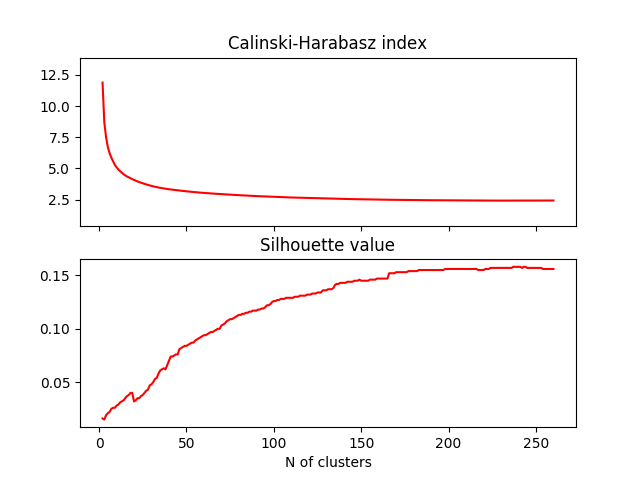
\includegraphics[width=9.5cm]{images/c-h-silh-index-plot-519-2_260-800-hierarchical.png}
    \caption{Hierarchical clustering. Calinski-Harabasz index and Silhoutte values for the
    manually annotated set of 455 publications clustered with hierarchical
    clustering, LSA with 800 components. The higher values denote 
    more compact and better clustering in both graphs.}
    \label{fig:ch-silh01}
  \end{center}
\end{figure}

\begin{figure}[ht]
  \begin{center}    
\includegraphics[width=9.5cm]{images/ari-plot-455-2_260-800-hierarchical.png}
    \caption{Hierarchical clustering. Adjusted Rand index for the
    manually annotated set of 455 publications clustered with hierarchical
    clustering, LSA with 800 components. The higher values denote 
    more compact and better clustering.}
    \label{fig:ari01}
  \end{center}
\end{figure}


In figure \ref{fig:ch-silh02}
we see corresponding graphs for k-means clustering. Top terms for
Calinski-Harabasz index maximum at seven clusters are listed in 
the Table \ref{table:topterms}.


\begin{figure}[ht]
  \begin{center}    
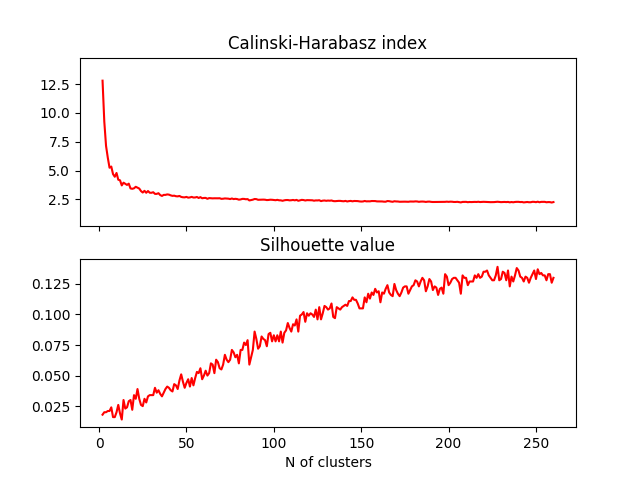
\includegraphics[width=9.5cm]{images/c-h-silh-index-plot-519-2_260-800-kmeans.png}
    \caption{k-means clustering. Calinski-Harabasz index and Silhoutte values for the
    manually annotated set of 455 publications clustered with k-means 
    clustering, LSA with 800 components. The higher values denote 
    more compact and better clustering in both graphs.}
    \label{fig:ch-silh02}
  \end{center}
\end{figure}

\begin{table}
\begin{tabular}{|p{2cm}|p{10.5cm}|} 
% Alignment of sells: l=left, c=center, r=right. 
% If you want wrapping lines, use p{width} exact cell widths.
% If you want vertical lines between columns, write | above between the letters
% Horizontal lines are generated with the \hline command:
\hline % The line on top of the table
\textbf{ } & \textbf{Top terms} \\ 
\hline 
\textbf{Cluster 0} & system internet management user project software architecture support decision business channel rule concept quality exercise  \\ 
\hline
\hline 
\textbf{Cluster 1} & lenges professional care intellectual disability people service special syndrome life child social support diagnosis pathology  \\ 
\hline
\hline 
\textbf{Cluster 2} & epilepsy stroke child seizure headache neuronal p rat sleep nerve risk treatment cell alcohol activity  \\ 
\hline
\hline 
\textbf{Cluster 3} & component filter signal neural linear bayesian ica feature value input simulation independent fuzzy vector output \\ 
\hline
\hline 
\textbf{Cluster 4} & dementia vascular ad cognitive stroke alzheimer diagnosis lesion vad risk pd brain impairment parkinson aneurysm \\ 
\hline
\hline 
\textbf{Cluster 5} & service development mobile switch agent system solution traffic environment protocol ip technology wireless game implementation \\ 
\hline
\hline 
\textbf{Cluster 6} & map image som self-organizing query logic document tree k expressive compression database retrieval rule cluster \\ 
\hline
\end{tabular} % for really simple tables, you can just use tabular
% You can place the caption either below (like here) or above the table
\caption{Top terms per cluster for manually annotated samples}
% Place the label just after the caption to make the link work
\label{table:topterms}
\end{table} % table makes a floating object with a title


\subsection{Precision and recall}
Recall is the number of items correctly classified divided by the 
total number of items in that class.
\begin{equation}
 Recall = \frac{|\{relevant\ items\} \cap \{retrieved\ items\}|} 
{\{relevant\ items\}}
\end{equation}

Precision is the number of items correctly classified divided by 
the total number items classified into that class (ie. true and 
false positives).
\begin{equation}
 Precision = \frac{|\{relevant\ items\} \cap \{retrieved\ 
items\}|} 
{\{retrieved\ items\}}
\end{equation}

With manually annotated dataset of 455 articles we compared 
the results with three clusters which was assumed the correct 
classification of the data set. We got recall $R = ???$ and 
precision $P = ???$ which is
a quite poor result. By looking at the top terms and random samples
from each cluster we notice that two of the three clusters have 
\emph{'Clinical neurology'} related items, see Tables
\ref{table:topterms_455_hier} and \ref{table:articles_455_hier}.

\begin{table}
\begin{tabular}{|p{2cm}|p{10.5cm}|} 
% Alignment of sells: l=left, c=center, r=right. 
% If you want wrapping lines, use p{width} exact cell widths.
% If you want vertical lines between columns, write | above between the letters
% Horizontal lines are generated with the \hline command:
\hline % The line on top of the table
\textbf{ } & \textbf{Top terms} \\ 
\hline 
\textbf{Cluster 1} & service image map system filter user som neural document mobile feature rule self-organizing logic query  \\ 
\hline
\hline 
\textbf{Cluster 2} & dementia vascular vad trial subcortical cognitive alzheimer criterion impairment cause lesion stroke subtypes prevalence ad  \\ 
\hline
\hline 
\textbf{Cluster 3} & stroke epilepsy pain treatment risk ad child seizure headache cognitive pd cortex parkinson cell apoe \\ 
\hline
\hline 
\end{tabular} % for really simple tables, you can just use tabular
% You can place the caption either below (like here) or above the table
\caption{Top terms for manually annotated dataset of 455 articles}
% Place the label just after the caption to make the link work
\label{table:topterms_455_hier}
\end{table} % table makes a floating object with a title

\begin{table}
\begin{tabular}{|c|p{6.5cm}|p{4.7cm}|} 
\hline % The line on top of the table
\textbf{ } & \textbf{Title} & \textbf{WoS category} \\ 
\hline 
\multirow{ 5}{*}{\textbf{1}} & Attacks against the WAP WTLS protocol & CS\_INFORMATION\_SYS \\
& Bringing knowing-when and knowing-what together: Periodically tuned categorizati & CS\_ARTIFICIAL\_INT  \\
& A digital television service architecture & CS\_INFORMATION\_SYS  \\ 
& A wavelet transform method for coding film-grain noise corrupted images & CS\_ARTIFICIAL\_INT  \\ 
& Accuracy of pedicle screw insertion with and without computer assistance: a rand & CLINICAL\_NEUROLOGY  \\
\hline
\hline 
\multirow{ 5}{*}{\textbf{2}} & Is subcortical vascular dementia a clinical entity for clinical drug trials? & CLINICAL\_NEUROLOGY \\
& Research criteria for subcortical vascular dementia in clinical trials & CLINICAL\_NEUROLOGY \\
& Subcortical vascular dementia as a specific target for clinical trials & CLINICAL\_NEUROLOGY \\ 
& Prognosis with dementia in Europe: A collaborative study of population-based coh & CLINICAL\_NEUROLOGY \\ 
& Comparison of different clinical criteria (DSM-III, ADDTC, ICD-10, NINDS-AIREN, & CLINICAL\_NEUROLOGY \\
\hline
\hline 
\multirow{ 5}{*}{\textbf{3}} & Interferon-alpha 2a effects on complement activation and regulation in MS patien & CLINICAL\_NEUROLOGY \\
& Architectural evolution - Nokia mobile phone case & CS\_INFORMATION\_SYS \\
& CASCADE: A European collaborative study on vascular determinants of brain lesion & PUBL\_ENVTL\_OCCUPA  \\ 
& Natural history of unruptured intracranial aneurysms: probability of and risk fa & CLINICAL\_NEUROLOGY \\ 
& An FDOPA PET study in patients with periodic limb movement disorder and restless & CLINICAL\_NEUROLOGY \\
\hline
\hline 
\end{tabular} % for really simple tables, you can just use tabular
\caption{Five random articles per cluster for manually annotated dataset of 455 articles}
\label{table:articles_455_hier}
\end{table} % table makes a floating object with a title



\subsection{Other metrics}
Different metrics to evaluate clustering include (from 
scikit-learn) Adjusted Rand Index, Mutual Information scores 
(NMI, AMI), homogenity, completness, V-measure, Fowlkes-Mallows 
scores, Silhouette Coefficient, Calinski-Harabaz Index, (from 
sources) 


%5.2 Finnish publications
\section{Finnish publications from year 2000}
We clustered year 2000 data, 10145 publications, with k-means 
clustering with different value of $k$, the number of clusters. 
The Figure \ref{fig:ch-silh02} shows the results.
\begin{figure}[ht]
  \begin{center}    
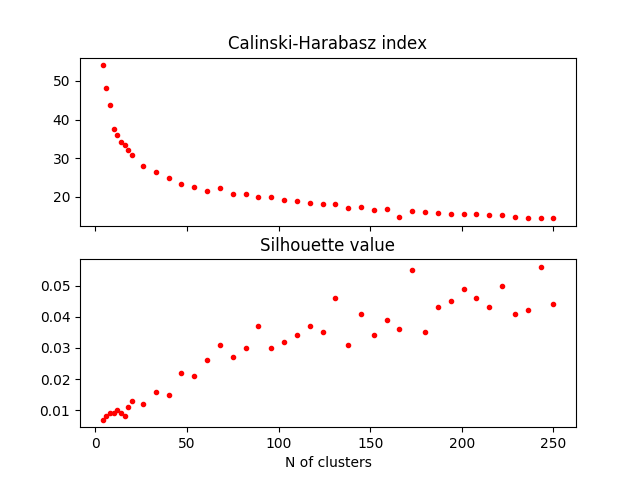
\includegraphics[width=10cm]{images/c-h-silh-index-plot-y2000-2_260-800-kmeans.png}
    \caption{Calinski-Harabasz index and Silhoutte values of 
10145 items clustered with k-means clustering, LSA with 800 
components. The higher values denote more compact and better 
clustering in both graphs.}
    \label{fig:ch-silh02}
  \end{center}
\end{figure}

Similarly the same data was clustered with agglomerative 
hierarchical Ward's clustering by sampling the number of clusters 
from the values [2-260]. The silhouette and Calinski-Harabasz values
are shown in Figure \ref{}
\begin{figure}[ht]
  \begin{center}    
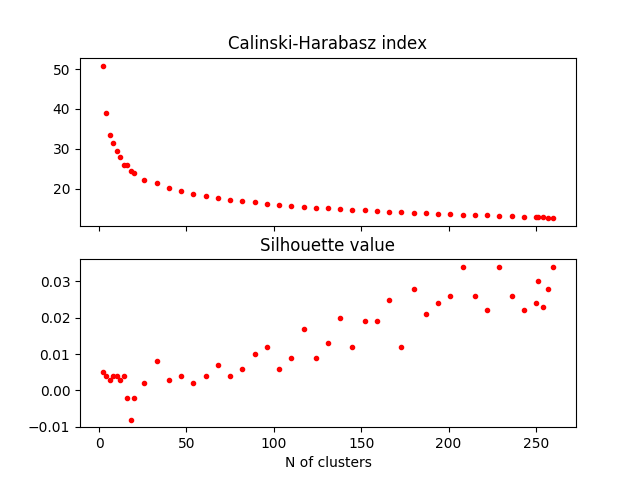
\includegraphics[width=10cm]{images/c-h-silh-index-plot-y2000-2_260-800-hierarchical.png}
    \caption{Hierarchical clustering. Calinski-Harabasz index and Silhoutte values for the
    Finnish publications from year 2000 clustered with hierarchical
    clustering, LSA with 800 components. The higher values denote 
    more compact and better clustering in both graphs.}
    \label{fig:ch-silh-2000-01}
  \end{center}
\end{figure}
We can see from the values that they prefer different features in
the data. Calinski-Harabasz index sees the fewest number of 
clusters - two - as the most compact and optimal clustering. Also
the form of the curve hints to perhaps power law that is also 
known as Zipf's law in text analysis. \fixme{Check this.}
It should be noticed that the silhouette values are quite low 
in absolute terms considering it's index space [-1,1]. This might 
be in line with the fact that it's best suited for [normally?] 
distributed and compact clusters. But we can also see that the 
silhouette values grow with the number of clusters although no
maxima seems to be reached with these cluster values.



% TODO: Kirjoita nämä oikeaan kohtaan tai poista
% Silhoutte values for 6000 publications clustered with 
% agglomerative clustering with Ward's method, number of clusters 
% 64, are seen in Figure~\ref{fig:silh01}.
% \begin{figure}[ht]
%   \begin{center}    
% 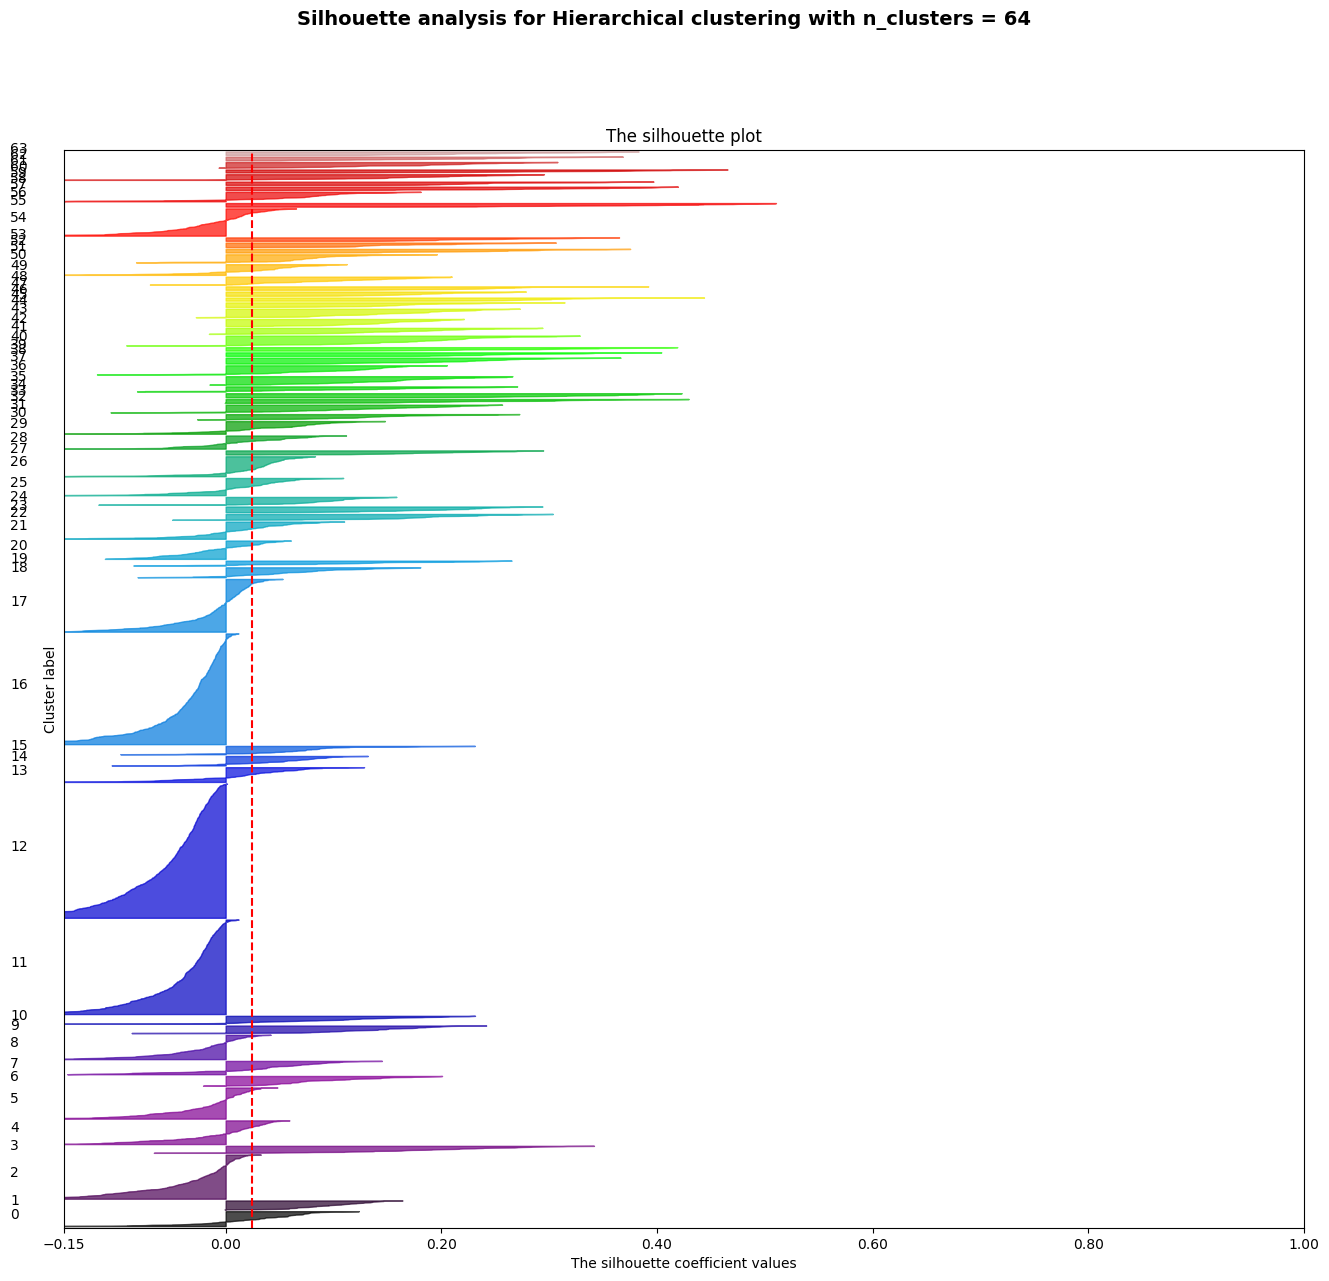
\includegraphics[width=13cm]{images/6000-64-400-Hierarchical-silhouette-plot.png}
%     \caption{Silhoutte values of 6000 items clustered with 
%     agglomerative clustering with Wrad's method, 64 clusters, 
%     LSA with 400 components. Each pixel row corresponds to a 
%     Silhouette value of an item, adjacent rows separated by gap 
%     corresponds to a cluster.
%     Dashed line is the average.}
%     \label{fig:silh01}
%   \end{center}
% \end{figure}
% 
% Other measure is Calinski-Harabaz index. Clustering should be 
% optimal when Calinski-Harabaz index reaches its maximum
% value~\cite{}.
% 
% When evaluating the results, Silhouette Coefficient might not be
% the best option. Find out why. V-measure or Adjusted Rand Index
% might be better options~\cite{noauthor_clustering_nodate}.






